\begin{figure}
    \centering
    \begin{subfigure}{0.41\linewidth}
        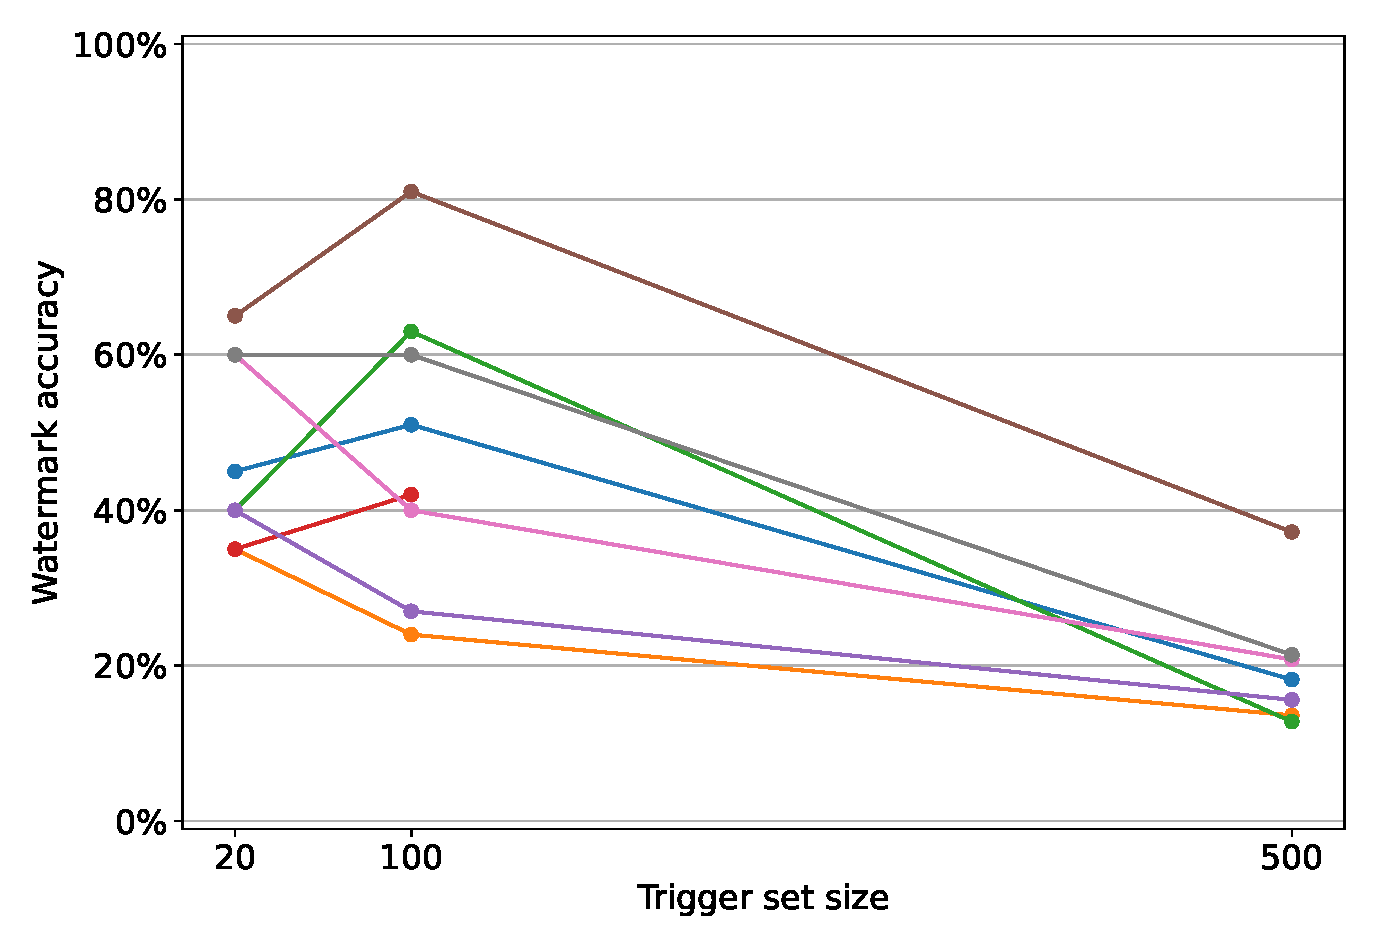
\includegraphics[width=\linewidth]{images/finetuning/densenet_finetuning_per_arch_00001.eps}
        \caption{DenseNet, fine-tuned with $\alpha=10^{-4}$}
        \label{fig:finetuning-smalllr-allmethods-perarch-densenet}
    \end{subfigure}
    \quad
    \begin{subfigure}{0.41\linewidth}
        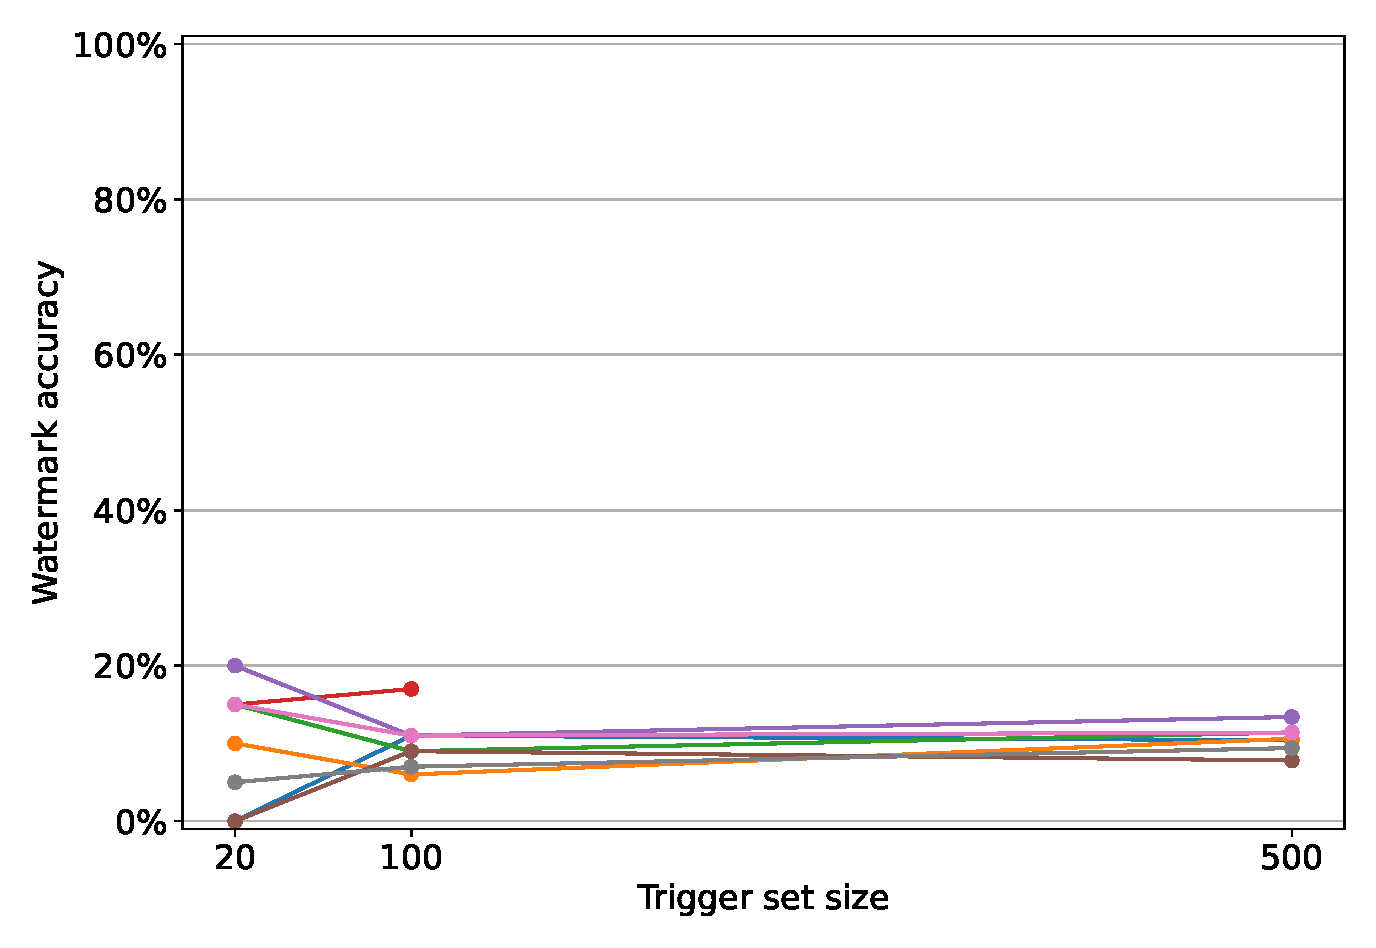
\includegraphics[width=\linewidth]{images/finetuning/densenet_finetuning_per_arch_001.eps}
        \caption{DenseNet, fine-tuned with $\alpha=10^{-2}$}
        \label{fig:finetuning-largelr-allmethods-perarch-densenet}
    \end{subfigure}
    \quad
    \begin{subfigure}{0.41\linewidth}
        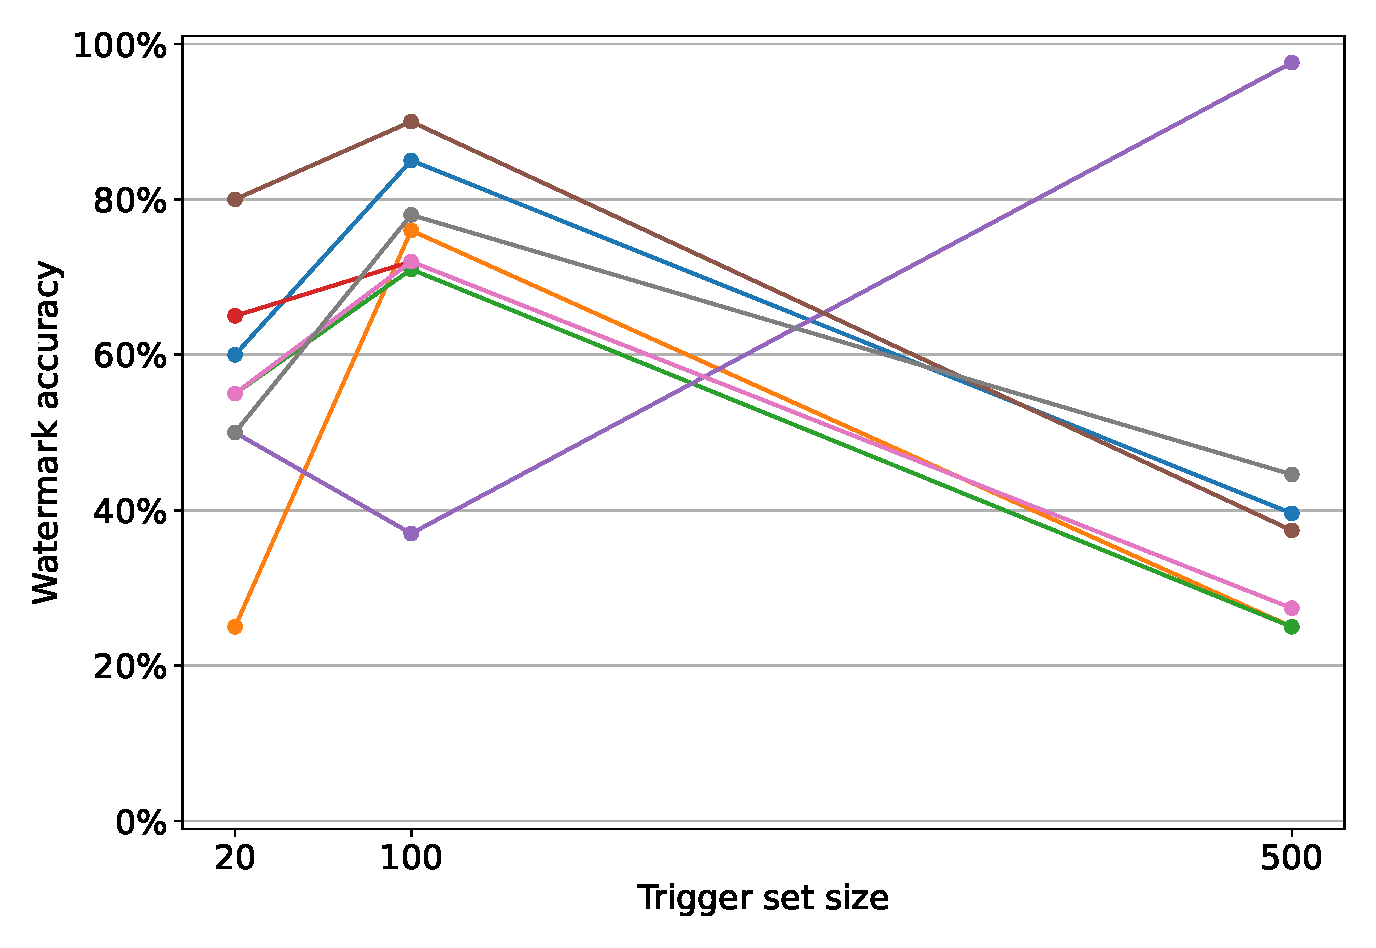
\includegraphics[width=\linewidth]{images/finetuning/resnet18_finetuning_per_arch_00001.eps}
        \caption{ResNet-18, fine-tuned with $\alpha=10^{-4}$}
        \label{fig:finetuning-smalllr-allmethods-perarch-resnet18}
    \end{subfigure}
    \quad
    \begin{subfigure}{0.41\linewidth}
        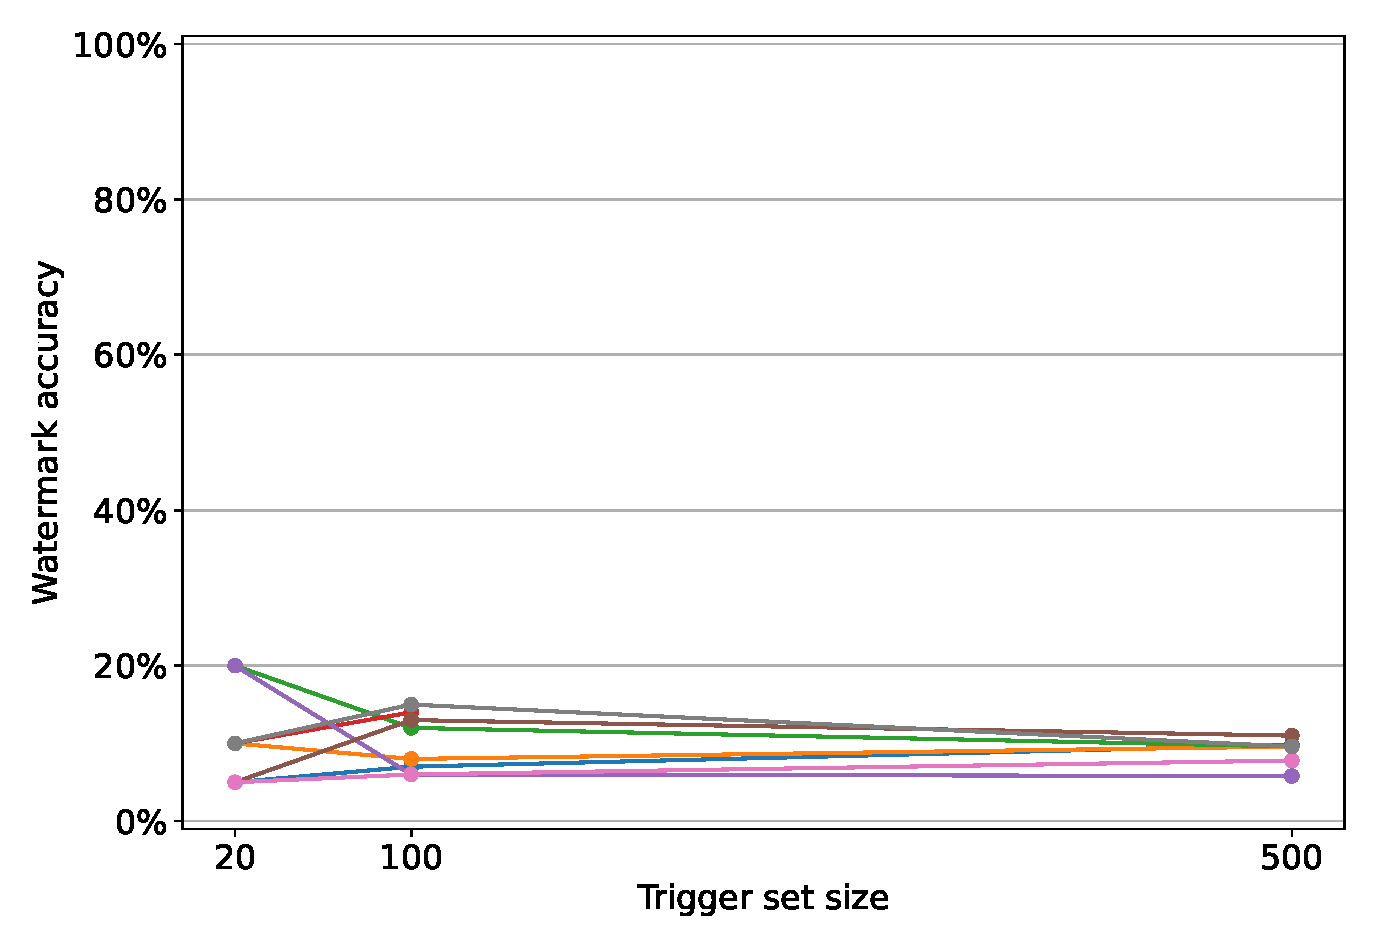
\includegraphics[width=\linewidth]{images/finetuning/resnet18_finetuning_per_arch_001.eps}
        \caption{ResNet-18, fine-tuned with $\alpha=10^{-2}$}
        \label{fig:finetuning-largelr-allmethods-perarch-resnet18}
    \end{subfigure}
    \quad
    \begin{subfigure}{0.41\linewidth}
        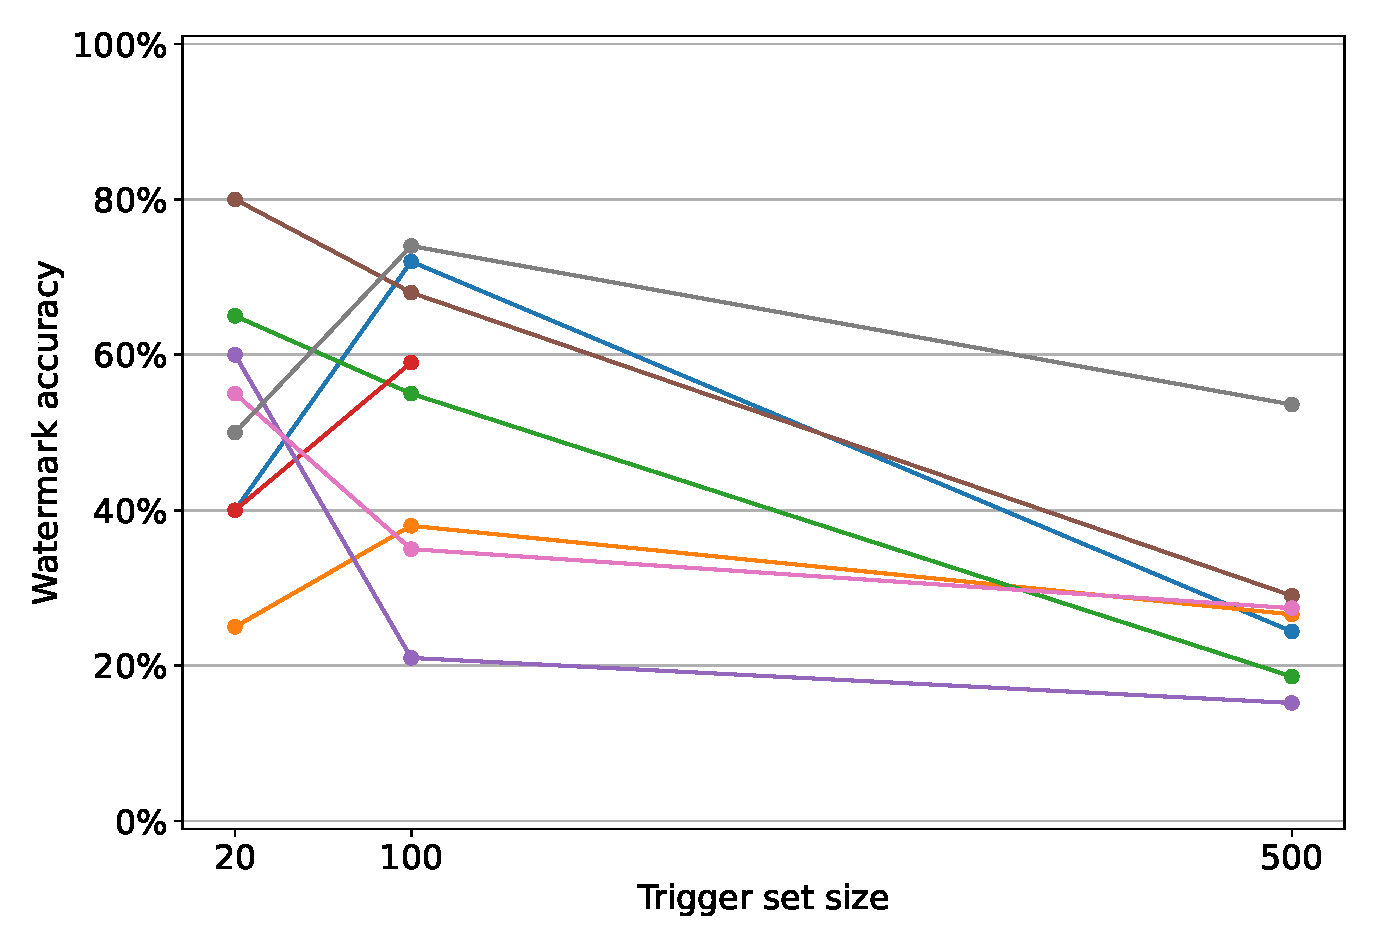
\includegraphics[width=\linewidth]{images/finetuning/resnet34_finetuning_per_arch_00001.eps}
        \caption{ResNet-34, fine-tuned with $\alpha=10^{-4}$}
        \label{fig:finetuning-smalllr-allmethods-perarch-resnet34}
    \end{subfigure}
    \quad
    \begin{subfigure}{0.41\linewidth}
        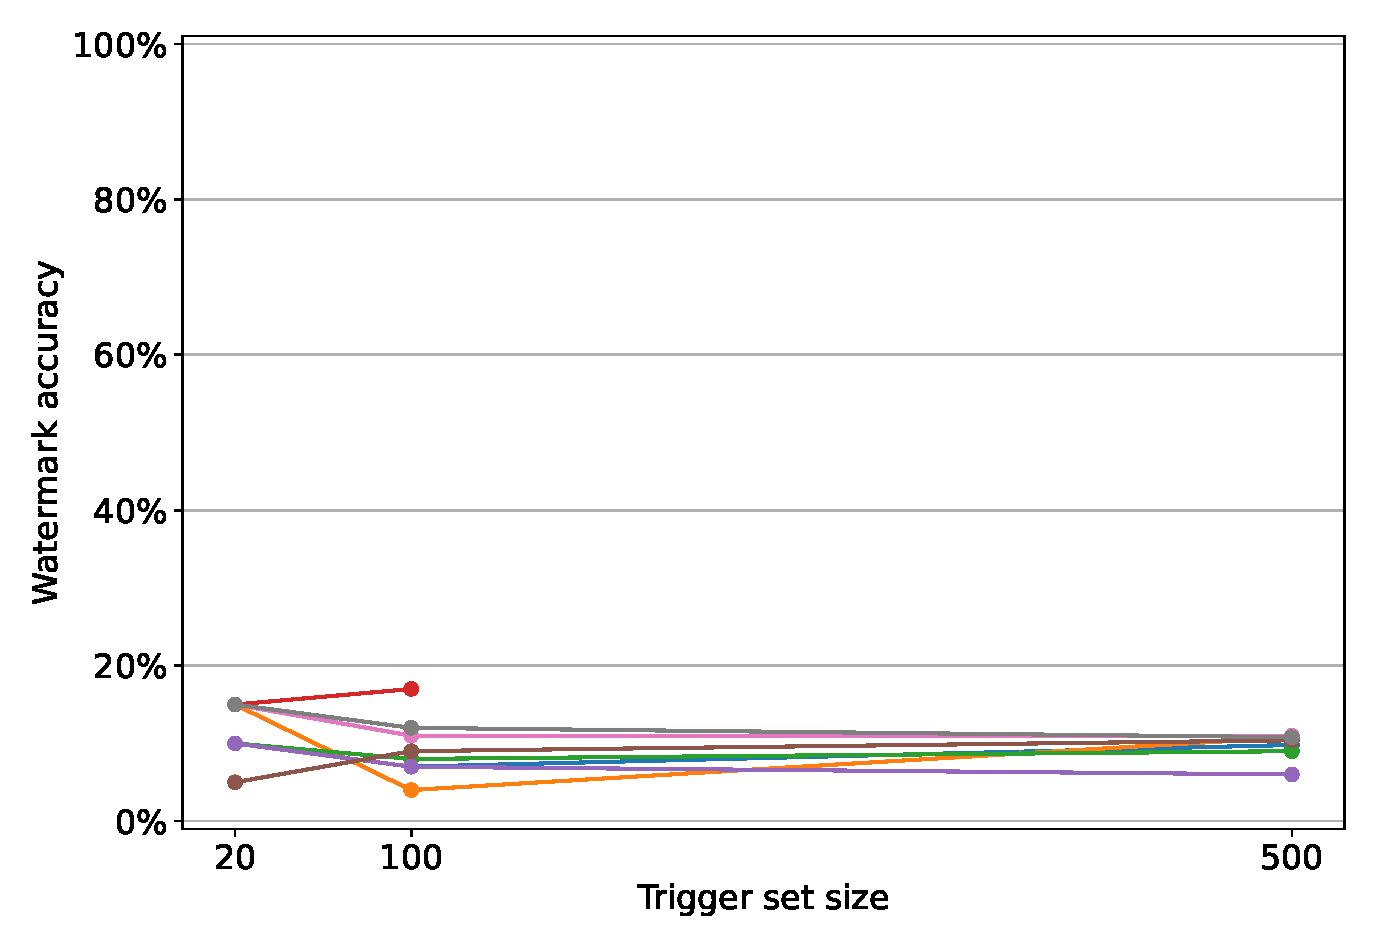
\includegraphics[width=\linewidth]{images/finetuning/resnet34_finetuning_per_arch_001.eps}
        \caption{ResNet-34, fine-tuned with $\alpha=10^{-2}$}
        \label{fig:finetuning-largelr-allmethods-perarch-resnet34}
    \end{subfigure}
    \quad
    \begin{subfigure}{0.41\linewidth}
        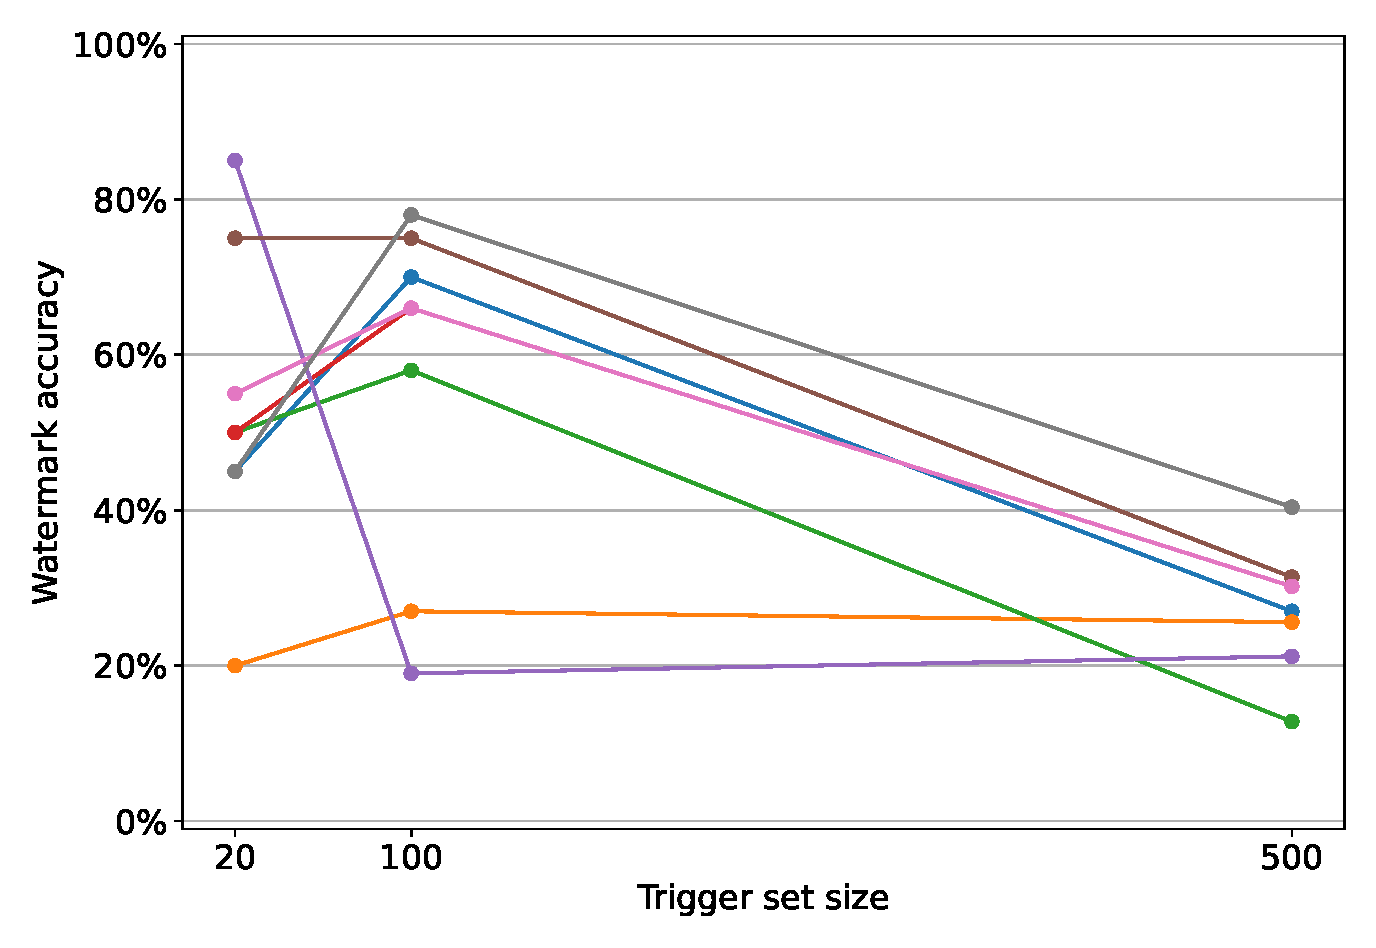
\includegraphics[width=\linewidth]{images/finetuning/resnet50_finetuning_per_arch_00001.eps}
        \caption{ResNet-50, fine-tuned with $\alpha=10^{-4}$}
        \label{fig:finetuning-smalllr-allmethods-perarch-resnet50}
    \end{subfigure}
    \quad
    \begin{subfigure}{0.41\linewidth}
        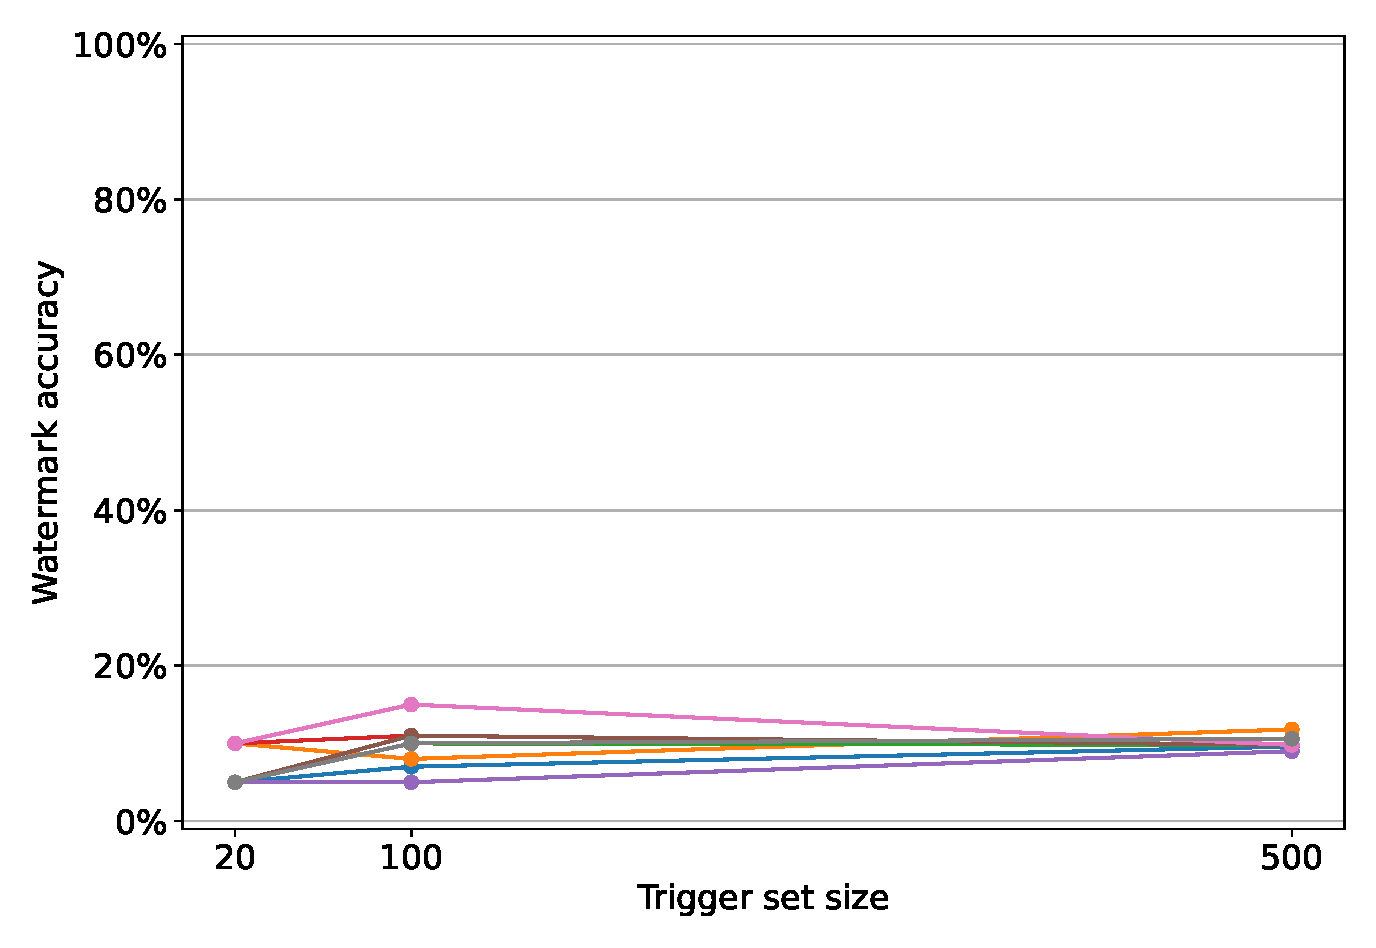
\includegraphics[width=\linewidth]{images/finetuning/resnet50_finetuning_per_arch_001.eps}
        \caption{ResNet-50, fine-tuned with $\alpha=10^{-2}$}
        \label{fig:finetuning-largelr-allmethods-perarch-resnet50}
    \end{subfigure}
    
    \begin{subfigure}{\linewidth}
    \centering
    
\includegraphics[height=1cm]{images/finetuning/legend_finetuning_per_arch_colors.eps}
    %\quad
    %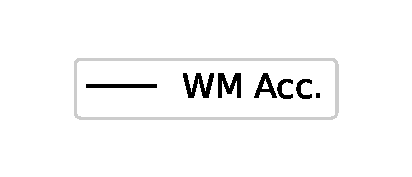
\includegraphics[height=1cm]{images/finetuning/legend_finetuning_per_arch_linestyles.eps}
    \end{subfigure}
    
    \caption{Influence of the trigger set size on robustness against fine-tuning on \textbf{CIFAR-10} models. Each plot on the right corresponds fine-tuning with a small learning rate and each plot on the left to fine-tuning with a large learning rate, all of them show the results for all watermarking methods.}
    \label{fig:finetuning-cifar10models-perarch}
\end{figure}
% The black dash-dotted line corresponds to the benchmark test accuracy of the non-watermarked model.
